% §IV Instrument (~1.25 pages, Fig. 3). Terminology FIXED here (EVIDENCE 혼용 금지):
%   "condition-forcing probe" = synthetic c-hat forcing (std/realistic 계열)
%   "state-transplant probe" = measured first-contact state injection (state-swap 계열)
%   "dose-response sweep"    = fcscale ramp 8/10/12N
%   "press simulation"       = closed-loop probe_press_sim
%   "live counterfactual probe" = on-robot frozen-obs
% Authority = % of mean commanded descent cancelled by the intervention.
% 08-11 수정: 용어 naive policy 통일; 각주 = 인스턴스 공시 전담 (RESULTS_LINEUP D 가드레일 ②);
% 서두를 prescription 프레임에 연결 ("recipe의 구조 절반이 instrument를 겸한다").
\section{The Conditioning Pathway}
\label{sec:method}

The pathway has two parts: a conditioning route built so that force reaches the action in one
explicit, calibrated form (\ref{sec:method-chat}--\ref{sec:method-mask}), and a battery of
counterfactual probes that measure how much that route moves the action
(\ref{sec:method-probes}). The route is designed to be \emph{drop-in} (no backbone change, no new
information), \emph{retrofittable} (attachable to a trained policy), and \emph{measurable}: because
it is explicit and unique, every component makes one number well-defined---how much does the
condition causally move the action?

\begin{figure}[t]
\centering
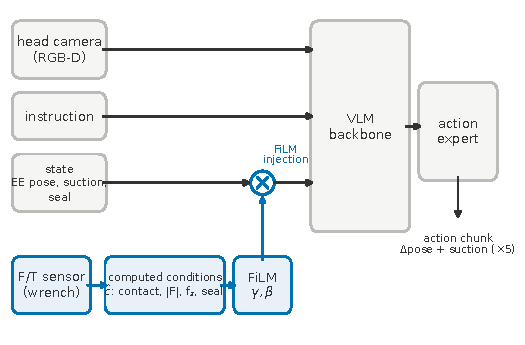
\includegraphics[width=\linewidth]{figs/architecture}
% 08-12 사용자 결정: mask는 그림에 미표기 — wrench가 state에 아예 없는 것으로 묘사
% (기능적으로 동등; mask 메커니즘은 §IV-C 본문이 설명).
\caption{The conditioned policy. The raw wrench does not enter the policy state; force reaches
the action only as the computed condition vector \chat{}, injected through FiLM modulation of
the state token entering the VLM backbone. Because this pathway is explicit and unique, forcing
\chat{} at inference measures the causal authority of the condition.}
\label{fig:arch}
\end{figure}

\subsection{Computed condition vector \chat{}}
\label{sec:method-chat}
From the wrench $F$ and seal bit already present in the naive policy's state we compute a small
set of task-critical conditions---the physical cues a human operator references (``if you feel
contact, stop; if the seal is on, lift''):
\begin{align}
\chat_{\mathrm{contact}} &= \mathrm{clip}\!\left(\left(\Fmag - F_0\right)/\tau,\ 0,\ 1\right),\nonumber\\
\chat_{\mathrm{fmag}} &= \left(\Fmag - F_0\right)/\tau_m \quad\text{(unsaturated)},\nonumber\\
\chat_{f_z} &= \left(f_z - o_z\right)/\tau_z,\qquad
\chat_{\mathrm{seal}} = \mathrm{seal},
\label{eq:chat}
\end{align}
with offsets and scales calibrated to the measured force statistics of the demonstrations (e.g.,
$F_0$ at the contact-onset magnitude).\footnote{Calibration quality matters and is itself a
finding. The conditioned policies in this paper are separately trained instances of the same
design: the robot picks (Sec.~\ref{sec:robot}) and the replication pair quoted in
Sec.~\ref{sec:offline-quintuple} use an earlier calibration; the recipe ablation and the live
counterfactuals (Sec.~\ref{sec:robot-live}) use offsets re-estimated from the measured contact
distribution plus the unsaturated $\chat_{\mathrm{fmag}}$ channel.} Two properties are essential. \emph{Computed, not
learned:} \chat{} is a fixed function of observed signals, so its physical meaning cannot drift
during training---which is what makes forcing \chat{} at inference a well-defined intervention
rather than a perturbation of an arbitrary latent. \emph{Zero new information:} every channel is a deterministic
function of state dimensions the naive policy also receives, so conditioning changes
\emph{routing}, never \emph{content}---the ``it works because it got extra sensing'' objection is
excluded by construction. The channels are deliberately plural: keeping contact, force magnitude,
and seal separate is what later lets the probes attribute authority to specific signals
(Sec.~\ref{sec:offline-posthoc}).

\subsection{FiLM injection and the force mask}
\label{sec:method-mask}
\chat{} enters the policy through FiLM modulation~\cite{perez2018film} at the state token
entering the VLM backbone; the injection site matters, and Sec.~\ref{sec:offline-pi0} compares
it against the action token.
% 09-15: "preliminary experiments" 각주 삭제 (사용자) — 근거는 §V-C π0 state vs action 비교로 대체.
The FiLM layer is zero-initialized so that it starts as the identity, and the backbone is
untouched: at the moment the pathway is attached, the conditioned policy \emph{is} the
already-trained policy, and can be fine-tuned in place from there. Every offline conditioned
policy in this paper is obtained this way, by continuing the trained naive checkpoint
(Sec.~\ref{sec:offline}).
The policy still receives the force information---only the structure of its delivery changes.
Because \chat{} is computed \emph{from} the wrench, leaving the raw wrench in the state would
hand the policy the same signal twice, once in each form; we therefore mask the wrench
dimensions from the state (Fig.~\ref{fig:arch}). Forcing \chat{} at inference then manipulates
\emph{all} of the force information the policy receives: if the policy responds to force at
all, it must show in how the action changes with \chat{}---the quantity the probes below
measure.

\subsection{Evaluation: counterfactual probe battery}
\label{sec:method-probes}
All probes intervene on a trained, frozen policy; none involves retraining. The offline probes
(P1--P4) run on held-out validation episodes. We define
\textbf{authority} as the intervention-induced change in the commanded vertical action on
committed-descent frames, expressed as a percentage of the mean commanded descent: $0\%$ means
the intervention is ignored, $100\%$ means it fully cancels descent, ${>}100\%$ means reversal
(retreat).

\textbf{(P1) Condition forcing (open loop).} How much does the condition alone move the
action? With images and state frozen, \chat{} is forced from its observed value to a target
pattern---either all channels saturated (\emph{full forcing}) or a calibrated contact-onset
pattern matching measured first-contact statistics (\emph{contact-moment forcing}). Applicable
to conditioned models only.

\textbf{(P2) State transplant (open loop).} Does the policy respond to a \emph{real}
contact state, and through which route? The six wrench dimensions of a measured first-contact
state (the median wrench at the first force rise, pooled over episodes; the seal bit keeps its
pre-contact value) are transplanted into pre-contact descent frames. This probe applies to any
policy, including the naive policy---it is what puts both policies on the same scale. Routing
the transplant selectively, to the \chat{} computation alone ($d_{\mathrm{FiLM}}$) or the raw
state alone ($d_{\mathrm{raw}}$), attributes the response to each route.

\textbf{(P3) Dose-response sweep.} Does the policy brake \emph{more} the harder it is
pressed? A policy that has bound braking to force should; one that has memorized a contact
template should respond most near the template and fade beyond it. The transplanted wrench is
rescaled to $8$, $10$, and $12$\,N and the response traced as a function of force \emph{dose};
since the demonstrations peak near the low end of this range, the upper doses measure
extrapolation. The sweep's \emph{slope sign} is the paper's central discriminator.

\textbf{(P4) Closed-loop press simulation.} Does the policy actually stop before the force
limit when no seal ever comes? Open-loop probes cannot show consequences, so we place the
frozen policy in a closed loop at each episode's nominal first-contact timing: commanded
descent advances a virtual penetration depth, a linear-stiffness force model raises the
simulated wrench accordingly, and the seal event is withheld---the operationally critical
misalignment scenario in which no press depth ever produces a seal. Outcomes: whether the
policy stops before the force limit, and maximum penetration. A control variant grants the seal
at a shallow depth, separating force-driven stopping from seal-event-driven stopping.

\textbf{(P5) Live counterfactual probe.} Do the offline responses hold on the real robot,
where the sensor, the contact, and the control loop are real rather than replayed or
simulated? We freeze observations at staged poses
along the approach and apply (P1)--(P3) interventions to \emph{two} policies---the conditioned
policy and the naive policy---on identical frozen observations, so both receive the same
physical counterfactual.

\textbf{Scope.} P1--P3 are single-frame and open-loop; P4 closes the loop under a force model;
P5 closes the gap to the real system. No single probe is decisive---the findings below rest on
their agreement.
